% ***************************************************
% Appendix
% ***************************************************
\chapter{Appendix}

\section{Repository}
The repository for this project can be found at \url{https://github.com/jdw5/metr4911}.

\section{Device Information}
\label{app:device_information}

\subsection{CPU Device Specifications}
\begin{table}[h]
    \centering
    \begin{tabular}{|l|l|}
        \hline
        \textbf{Component} & \textbf{Specification} \\
        \hline
        Architecture & x86\_64 \\
        CPU Cores & 8 \\
        CPU Frequency & 3100 MHz \\
        System RAM & 90 GB Total \\
        GPU & N/A \\
        GPU Memory & N/A \\
        \hline
    \end{tabular}
    \caption{System Specifications for CPU Test Environment}
    \label{tab:cpu_specs}
\end{table}

\subsection{P100 Device Specifications}
\begin{table}[h]
    \centering
    \begin{tabular}{|l|l|}
        \hline
        \textbf{Component} & \textbf{Specification} \\
        \hline
        Architecture & x86\_64 \\
        CPU Cores & 20 (Physical) / 20 (Total) \\
        CPU Frequency & 3012.026 MHz \\
        System RAM & 251.55 GB Total \\
        GPU & Tesla P100-PCIE-16GB \\
        GPU Memory & 15.90 GB \\
        \hline
    \end{tabular}
    \caption{Device Specifications for P100 test environment}
    \label{tab:p100_specs}
\end{table}

\subsection{A100 Device Specifications}
\begin{table}[h]
    \centering
    \begin{tabular}{|l|l|}
        \hline
        \textbf{Component} & \textbf{Specification} \\
        \hline
        Architecture & x86\_64 \\
        CPU Cores & 8 \\
        CPU Frequency & 2894.562 MHz \\
        System RAM & 93.88 GB Total \\
        GPU & NVIDIA A100-PCIE-40GB \\
        GPU Memory & 39.39 GB \\
        \hline
    \end{tabular}
    \caption{Device Specifications for A100 test environment}
    \label{tab:a100_specs}
\end{table}


\section{Convolution Results}

\subsection{CPU}
\begin{table}[h]
    \centering
    \begin{tabular}{|c|c|}
        \hline
        \textbf{Test Number} & \textbf{Execution Time (ns)} \\
        \hline
        1 & 213342 \\
        2 & 223891 \\
        3 & 229782 \\
        4 & 249048 \\
        5 & 252755 \\
        \hline
    \end{tabular}
    \caption{CPU Convolution Execution Times}
    \label{tab:cpu_conv_times}
\end{table}

\textbf{Test Configuration:}
\begin{itemize}
    \item Input Size: 8 x 8 x 1
    \item Kernel Size: 2 x 2 x 1 x 10
    \item Output Feature Size: 7 x 7 x 10
    \item Resolution: 8-bit
    \item Stride Steps: 1
    \item Zero Padding: 0
\end{itemize}

\subsection{P100}
\begin{table}[h]
    \centering
    \begin{tabular}{|c|c|}
        \hline
        \textbf{Test Number} & \textbf{Execution Time (ns)} \\
        \hline
        1 & 1010.27 \\
        3 & 1016.85 \\
        3 & 1020.45 \\
        4 & 1056.34 \\
        5 & 1120.34 \\
        \hline
    \end{tabular}
    \caption{A100 Convolution Execution Times}
    \label{tab:a100_conv_times}
\end{table}

% You might want to add these statistics
\textbf{Test Configuration:}
\begin{itemize}
    \item Input Size: 8 x 8 x 1
    \item Kernel Size: 2 x 2 x 1 x 10
    \item Output Feature Size: 7 x 7 x 10
    \item Resolution: 8-bit
    \item Stride Steps: 1
    \item Zero Padding: 0
\end{itemize}

\subsection{A100}
\begin{table}[h]
    \centering
    \begin{tabular}{|c|c|}
        \hline
        \textbf{Test Number} & \textbf{Execution Time (ns)} \\
        \hline
        1 & 608.35 \\
        2 & 608.73 \\
        3 & 610.98 \\
        4 & 612.70 \\
        5 & 613.58 \\
        \hline
    \end{tabular}
    \caption{P100 Convolution Execution Times}
    \label{tab:p100_conv_times}
\end{table}

\textbf{Test Configuration:}
\begin{itemize}
    \item Input Size: 8 x 8 x 1
    \item Kernel Size: 2 x 2 x 1 x 10
    \item Output Feature Size: 7 x 7 x 10
    \item Resolution: 8-bit
    \item Stride Steps: 1
    \item Zero Padding: 0
\end{itemize}

\newpage
\section{HDL Type Primitive}
\label{app:hdl_type_primitive}

A custom hardware type primitive was created for this project. 
It represents a feature with a height, width and depth to simplify the hardware design.

\begin{lstlisting}[language=VHDL]
type feature_t is array(natural range <>, natural range <>, natural range <>) of signed;
\end{lstlisting}

\section{Schematics}
The below pages are the hardware schematics for the project.
These are provided at high resolution to allow for detailed inspection.
The first page provided is the accelerator component, which describes the linking of the generic layers.
The second schematic is the accelerator connected to block RAMs to pass the weights and bias signals. It wraps the accelerator in a block RAM interface.
The third schematic is the system on chip, which receives the input image from the NeoRV32 softcore processor. It implements the previous schematic as an IP core.

\newpage
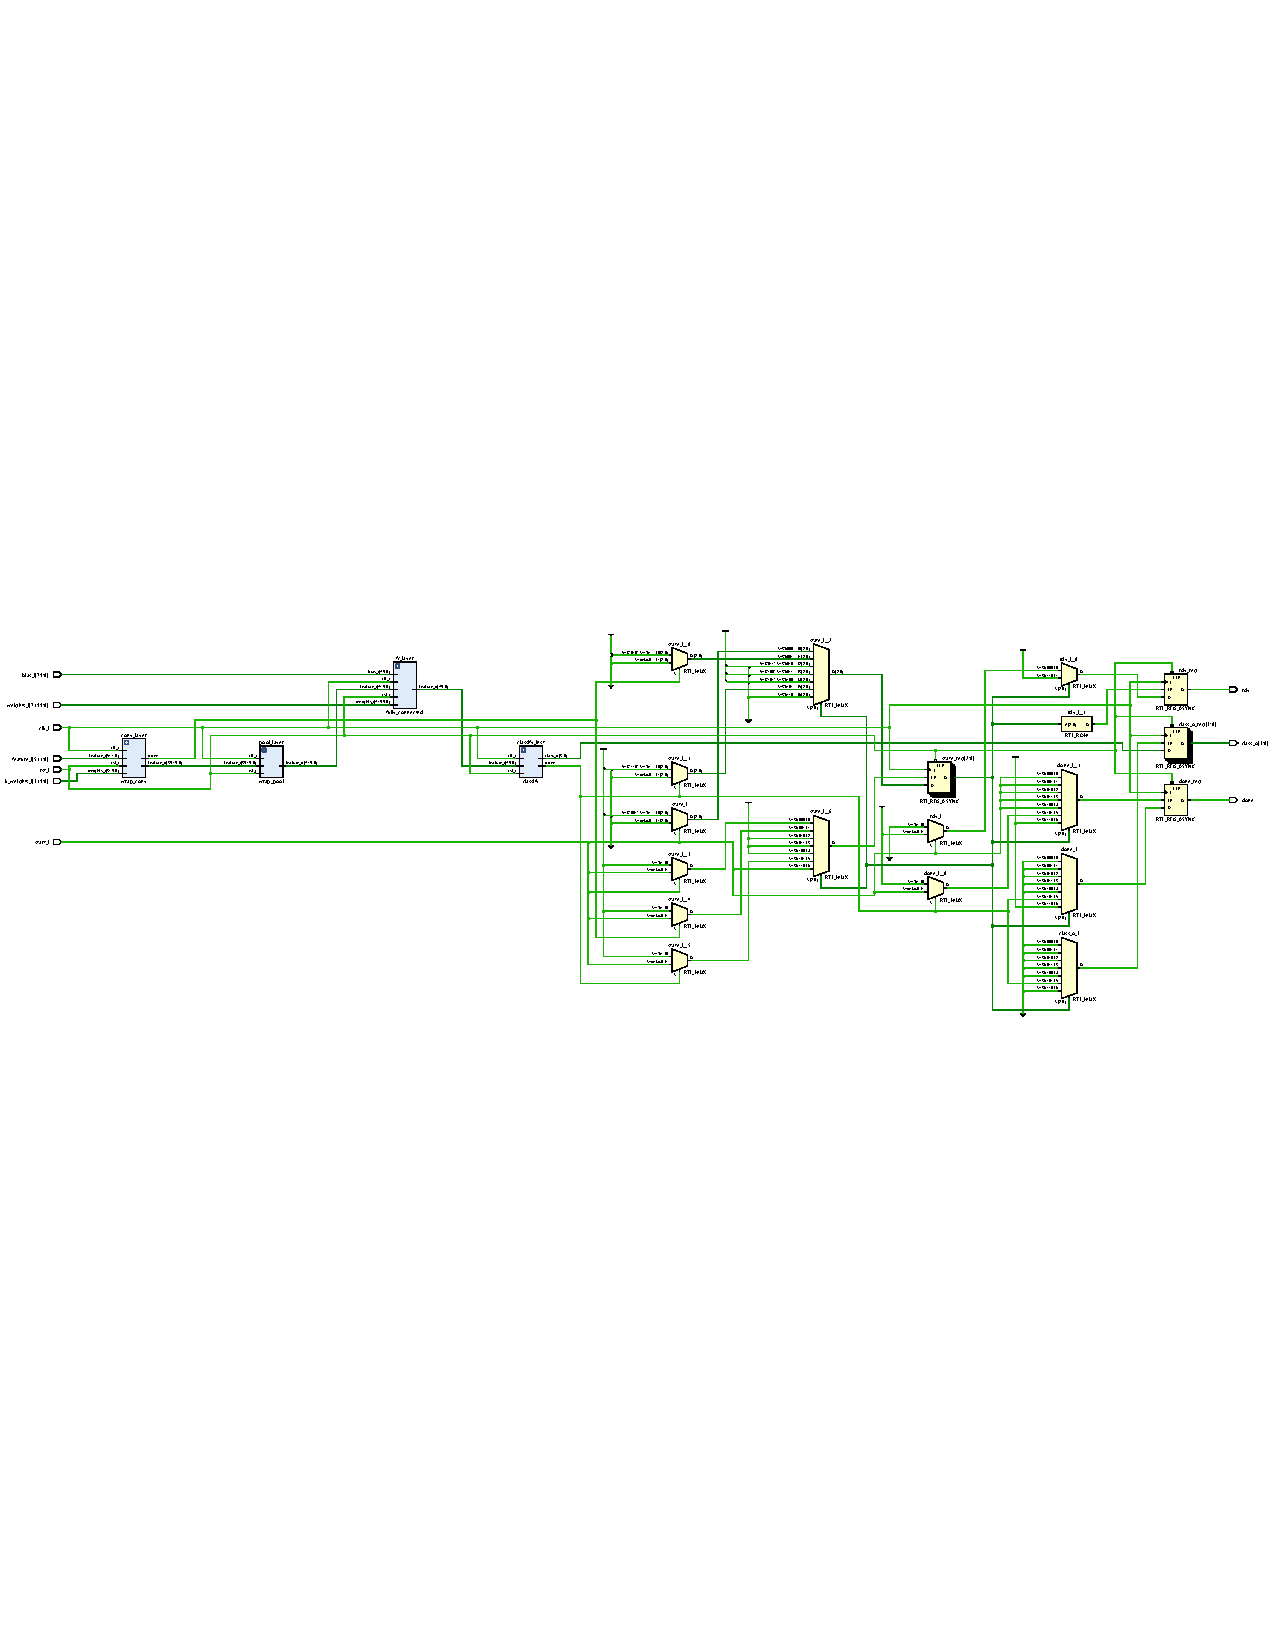
\includepdf[pages=-]{Figs/accelerator.pdf}

\newpage
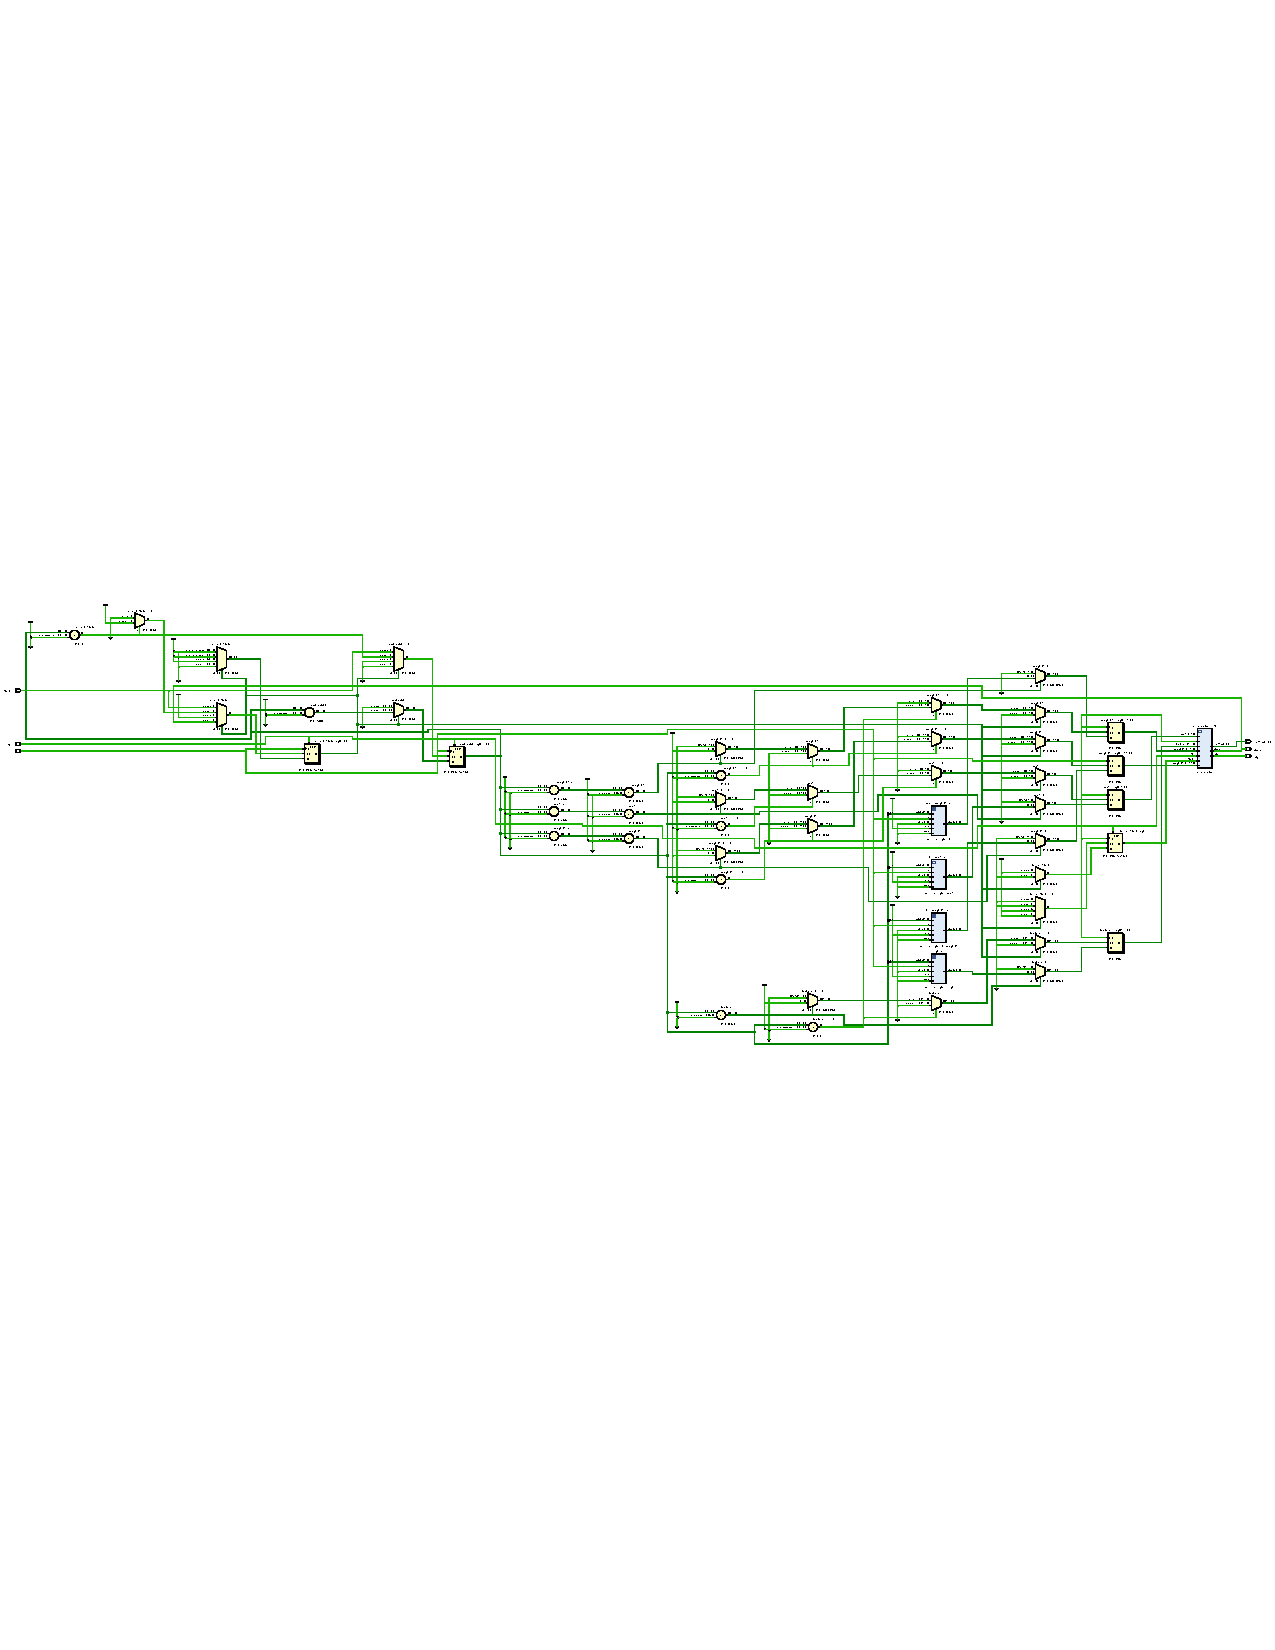
\includepdf[pages=-]{Figs/mem_accelerator.pdf}

\newpage
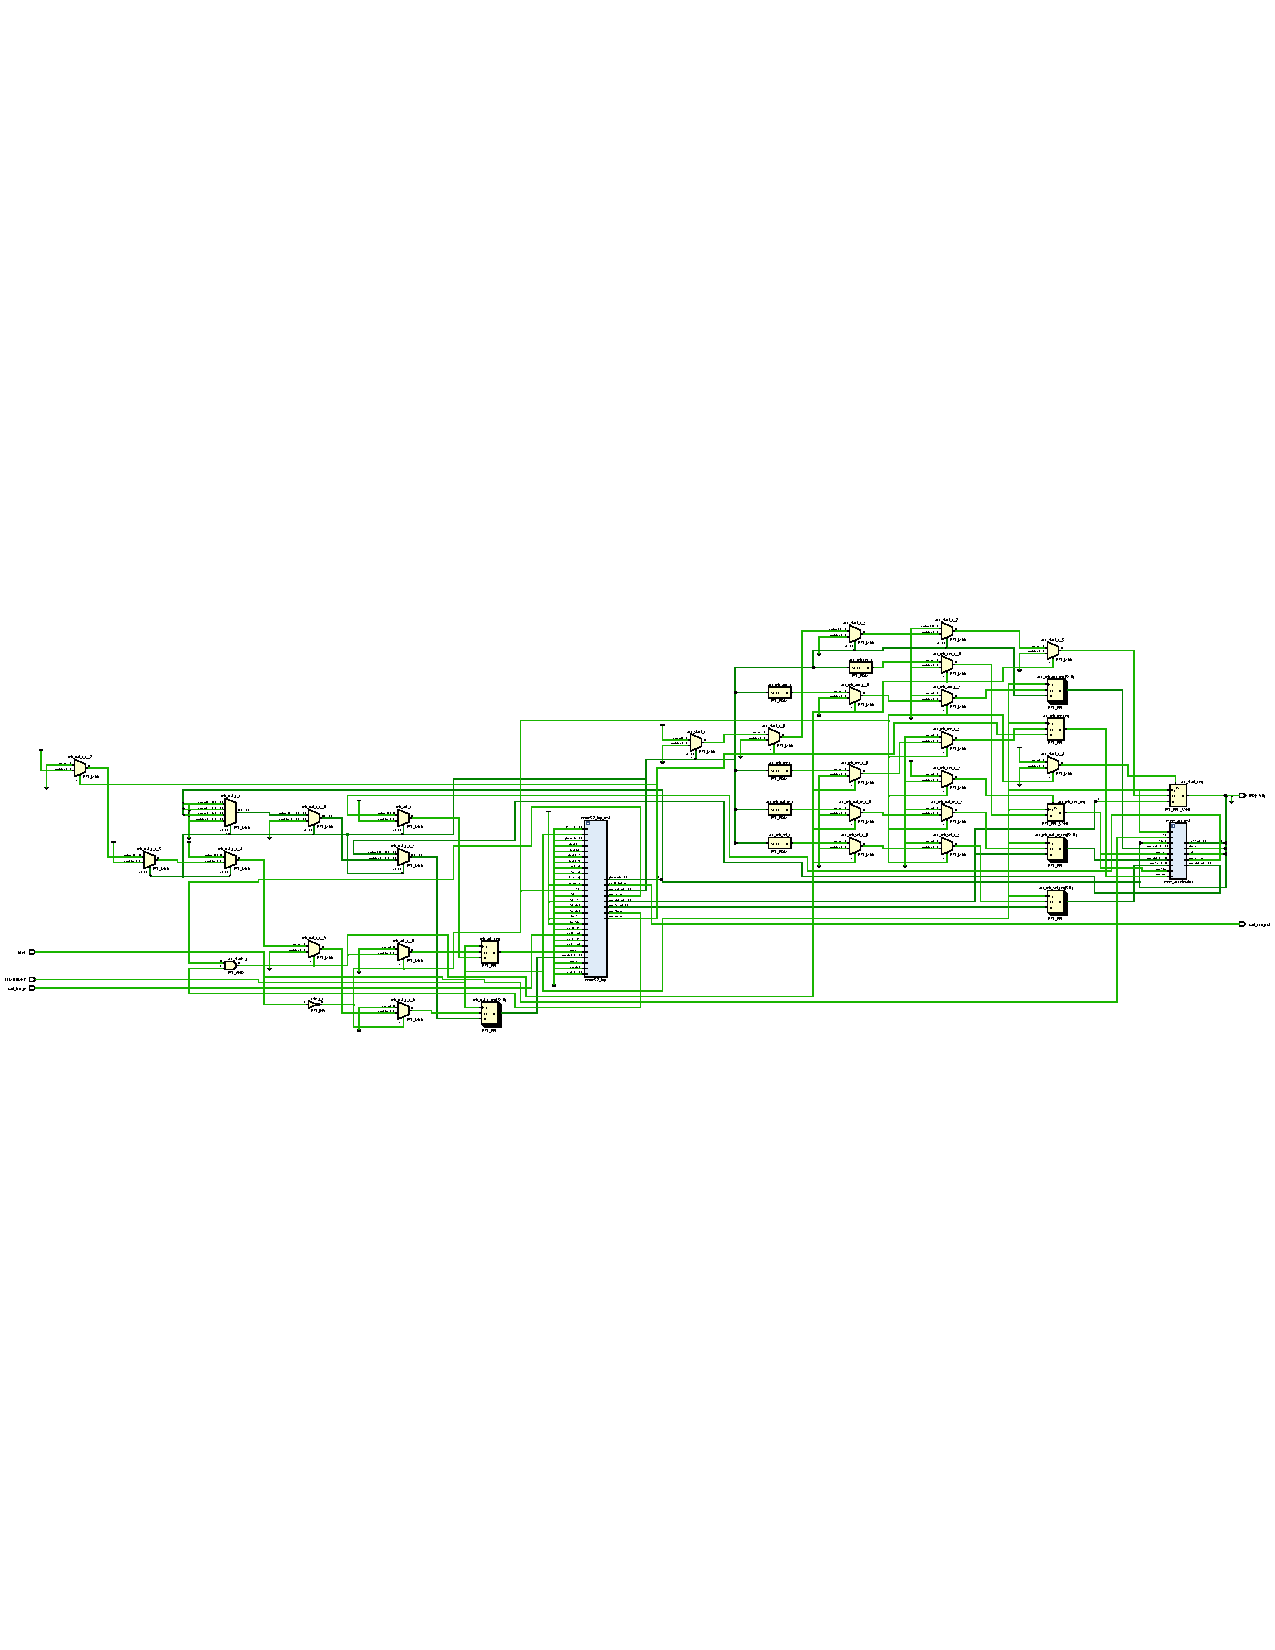
\includepdf[pages=-]{Figs/riscv-ml-core.pdf}
